\documentclass[main.tex]{subfiles}

\begin{document}

\section{Sampling the Full Medium Splitting Functions}\label{app: medium_MetropolisHastings}
This appendix will give the procedures for sampling random values from the full medium splitting functions by use of Metropolis-Hastings algorithm. The splitting functions for the three vertices are given to leading logarithmic accuracy by \cite{Universal_quark_gluon_ratio_in_medium-induced_parton_cascade}
\begin{align}
    \mathcal{K}_{gg}(z) &= \frac{1}{2} 2 C_A \, \frac{[1-z(1-z)]^2}{z(1-z)} \, \sqrt{\frac{(1-z)C_A + z^2 C_A}{z(1-z)}} \label{eqn: medium_full_splittingfunctions_gg} \\
    \mathcal{K}_{qg}(z) &= \frac{1}{2} 2 N_f \, T_F \, \left(z^2 +(1-z)^2)\right) \, \sqrt{\frac{C_F - z(1-z)C_A}{z(1-z)}} \label{eqn: medium_full_splittingfunctions_qg} \\
    \mathcal{K}_{qq}(z) &= \frac{1}{2} C_F \, \frac{1+z^2}{(1-z)} \, \sqrt{\frac{zC_A + (1-z)^2 C_F}{z(1-z)}}. \label{eqn: medium_full_splittingfunctions_qq}
\end{align}
The color factors on the outside of the square roots will be disregarded in the calculations, as these will cancel out, but we will keep the color factors inside the square roots (which we usually absorb into \(\hat q\), as they have some impacts on the shape of the distributions. We could set \(C_A=C_F=1\), and the algorithms presented here would still sample correctly, but the shape would be slightly different. 

\subsection*{The \(gg\) vertex}
The full ggg splitting kernel is given by \autoref{eqn: medium_full_splittingfunctions_gg}.
To generate a random value from this function, we need to go back to the Metropolis-Hastings algorithm. 
For this we need a proportional dummy-function, we can use the simplified kernel given by \autoref{eqn: ggg_medium_reduced_kernel}, the integral can be generally shown to be, 
\begin{align}
    \int \mathcal{K}_{gg}^{\text{dummy}}(z)\,dz = \int \frac{2}{(z(1-z))^{3/2}}\,dz &= 2\,\frac{4z-2}{\sqrt{-z(z-1)}}.
\end{align}
Sampling random momentum fractions for the distribution is again done by solving \autoref{eqn: energyfraction_function_R}
\begin{align}
    \mathcal{R}\, \int_{\epsilon}^{1-\epsilon} \mathcal{K}_{gg}^{\text{dummy}}(z)\,dz &= \int_{\epsilon}^{y} \mathcal{K}_{gg}^{\text{dummy}}(z)\,dz \nonumber \\
    \mathcal{R}\, \int_{\epsilon}^{1-\epsilon} \mathcal{K}_{gg}^{\text{dummy}}(z)\,dz &= 2\,\frac{4y-2}{\sqrt{-y(y-1)}} - 2\,\frac{4\epsilon-2}{\sqrt{-\epsilon(\epsilon-1)}} \nonumber\\
    \frac{\mathcal{R}}{2}\, \int_{\epsilon}^{1-\epsilon} \mathcal{K}_{gg}^{\text{dummy}}(z)\,dz + \frac{4\epsilon-2}{\sqrt{\epsilon(1-\epsilon)}} &= \frac{4y-2}{\sqrt{y(1-y)}} \nonumber\\
    \frac{1}{2}\, \int_{\epsilon}^{1-\epsilon} \mathcal{K}_{gg}^{\text{dummy}}(z)\,dz \left(\mathcal{R}-\frac{1}{2} \right) &= \frac{4y-2}{\sqrt{y(1-y)}}.
\end{align}
Reinserting the initial factors of the integral, by setting \( a= \frac{1}{2}\, \int_{\epsilon}^{1-\epsilon} \mathcal{K}_{gg}^{\text{dummy}}(z)\,dz \left(\mathcal{R}-\frac{1}{2} \right)\), this equation can be solved using Mathematica,
\begin{align}\label{eqn: sampling_p_ggg_medium}
    y &= \frac{16 + a^2 \mp a \sqrt{16 + a^2}}{2 (16 + a^2)} \nonumber\\
    y &= \frac{1}{2} \mp \frac{a \sqrt{16 + a^2}}{2 (16 + a^2)} \nonumber\\
    y &= \frac{1}{2} \mp \frac{a }{2 \sqrt{16 + a^2}}.
\end{align}
We now have a method for randomly drawing a sample from the dummy splitting function, and can follow the procedure of \autoref{sec: metropolis_hastings} to implement \autoref{eqn: sampling_p_ggg_medium} into a MH algorithm to draw samples from the full splitting function. The plots of the original histogram, and MH corrected histogram is given in \autoref{fig: MH_corrected_k_gg_medium_splitting}.
\begin{figure}[hbt]
    \centering
    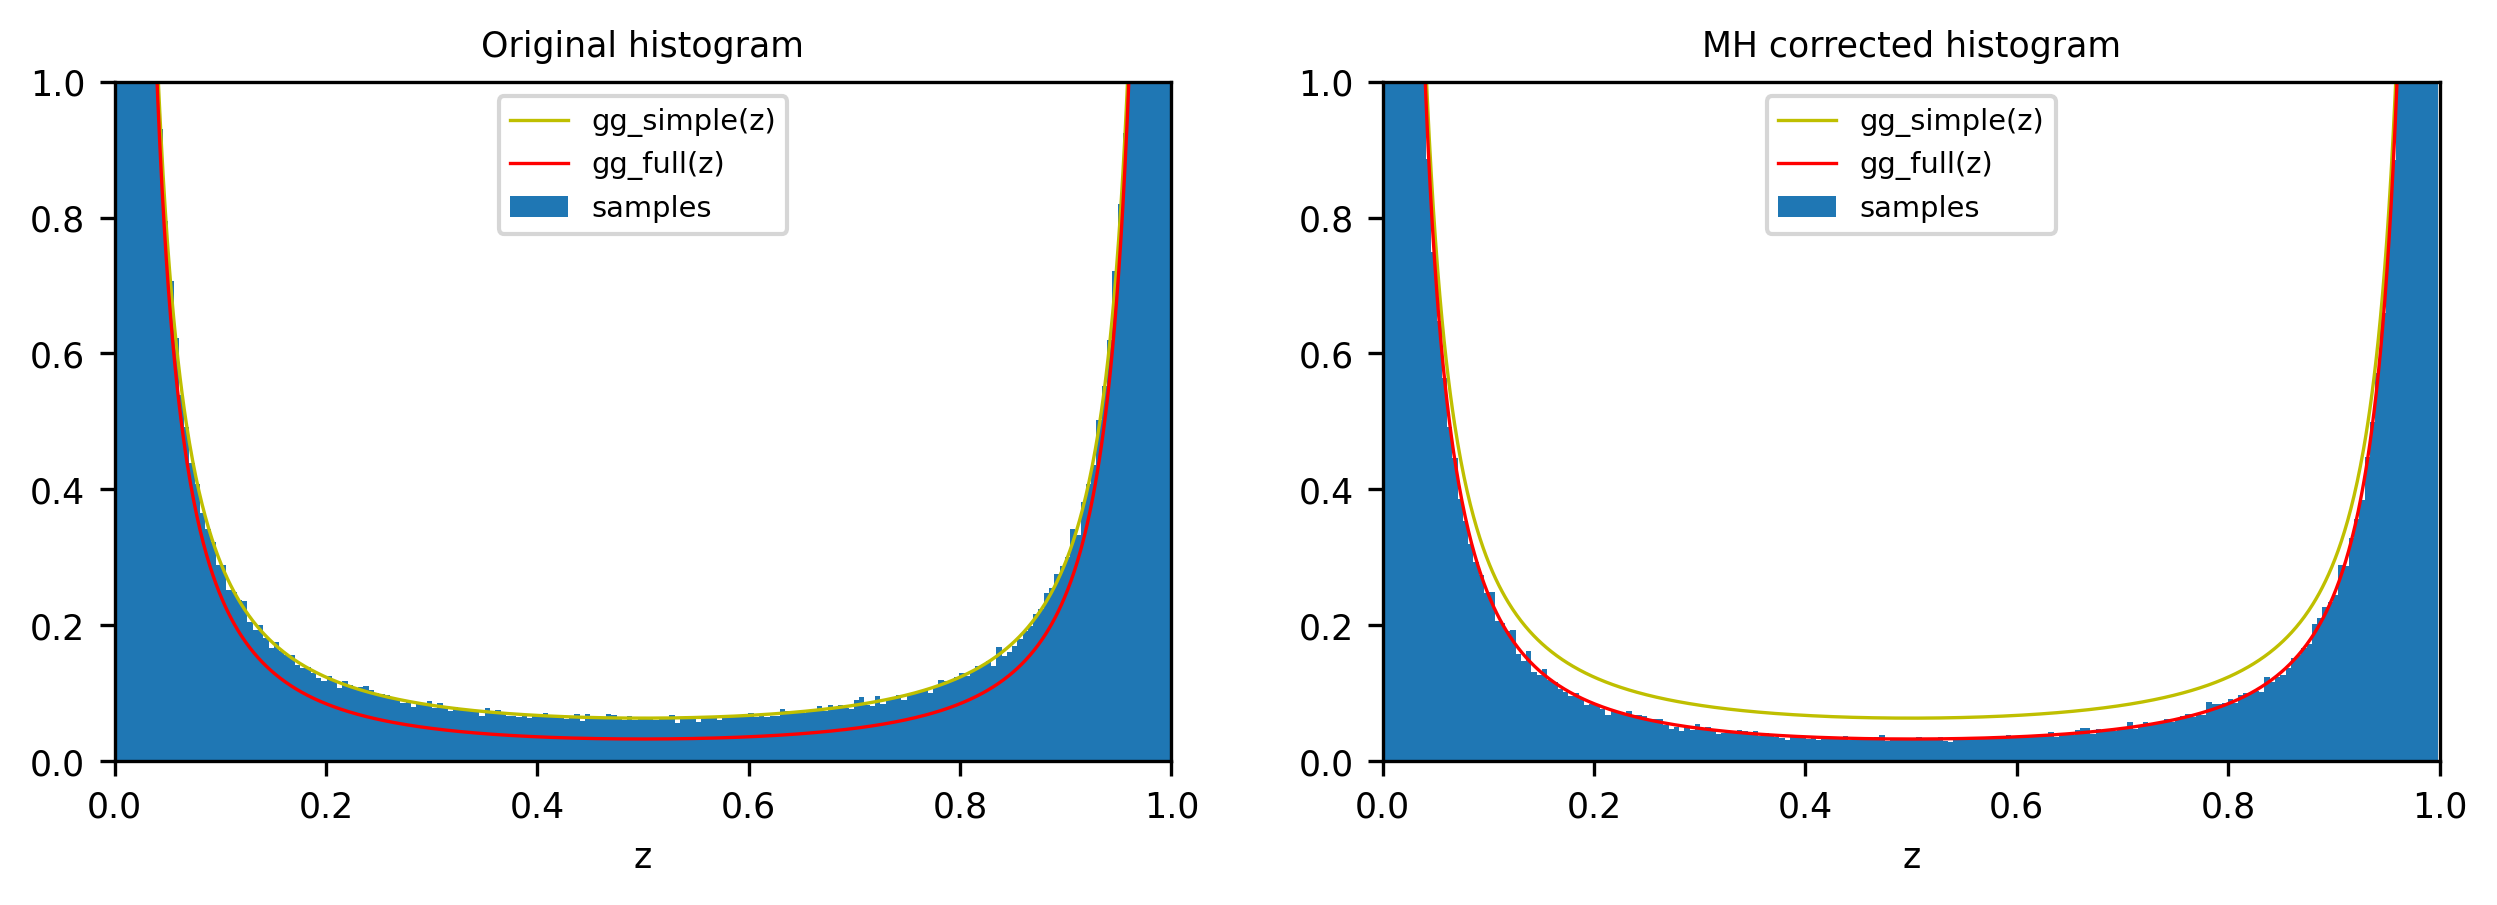
\includegraphics[width=15cm]{pictures/plots/Metropolis-Hastings/MH_medium_gg.png}
    \caption{Probability density of the medium \(\mathcal{K}_{gg}\) splitting function, compared to the histogram of the dummy splitting function, and the Metropolis-Hastings corrected results. Simulated with \(1,000,000\) points, and an acceptance rate of \(0.82\).}
    \label{fig: MH_corrected_k_gg_medium_splitting}
\end{figure}

\subsection*{The \(qg\) vertex}
Continuing now with the \(qg\) splitting function, \autoref{eqn: medium_full_splittingfunctions_qg}. With some inspiration from the previous section, we can propose the following dummy function
\begin{equation}
    \mathcal{K}_{qg}^{\text{dummy}}(z) = \frac{1}{\sqrt{z (1-z)}}
\end{equation}
whose integral can be shown to be, 
\begin{align}
    \int \mathcal{K}_{qg}^{\text{dummy}}(z) \, dz = \int \frac{1}{\sqrt{z(1-z)}}\, dz &= -2 \sin^{-1}(\sqrt{1-z}).
\end{align}
When evaluating \autoref{eqn: energyfraction_function_R} we get
\begin{align}
    \mathcal{R} \int_\epsilon^{1-\epsilon} \mathcal{K}_{qg}^{\text{dummy}}(z)\,dz  &= \int_\epsilon^{y} \mathcal{K}_{qg}^{\text{dummy}}(z)\,dz  \nonumber\\
    \mathcal{R} \int_\epsilon^{1-\epsilon} \mathcal{K}_{qg}^{\text{dummy}}(z)\,dz &= -2 \sin^{-1}(\sqrt{1-y}) + 2 \sin^{-1}(\sqrt{1-\epsilon}) \nonumber\\
    -\mathcal{R} \int_\epsilon^{1-\epsilon} \mathcal{K}_{qg}^{\text{dummy}}(z)\,dz + 2 \sin^{-1}(\sqrt{1-\epsilon}) &= 2 \sin^{-1}(\sqrt{1-y}) 
\end{align}
setting \(a = -\mathcal{R} \int_\epsilon^{1-\epsilon} \mathcal{K}_{qg}^{\text{dummy}}(z)\,dz + 2 \sin^{-1}(\sqrt{1-\epsilon})\), and finally solving for y
\begin{align}\label{eqn: sampling_p_gqq_medium}
    a &= 2 \sin^{-1}(\sqrt{1-y}) \nonumber\\
    y &= 1- \left(\sin (\frac{a}{2})\right)^2.
\end{align}
Using \autoref{eqn: sampling_p_gqq_medium} to sample values for the dummy function, we can run the MH algorithm as in previous sections and obtain \autoref{fig: MH_corrected_k_qg_medium_splitting}.
\begin{figure}[htb]
    \centering
    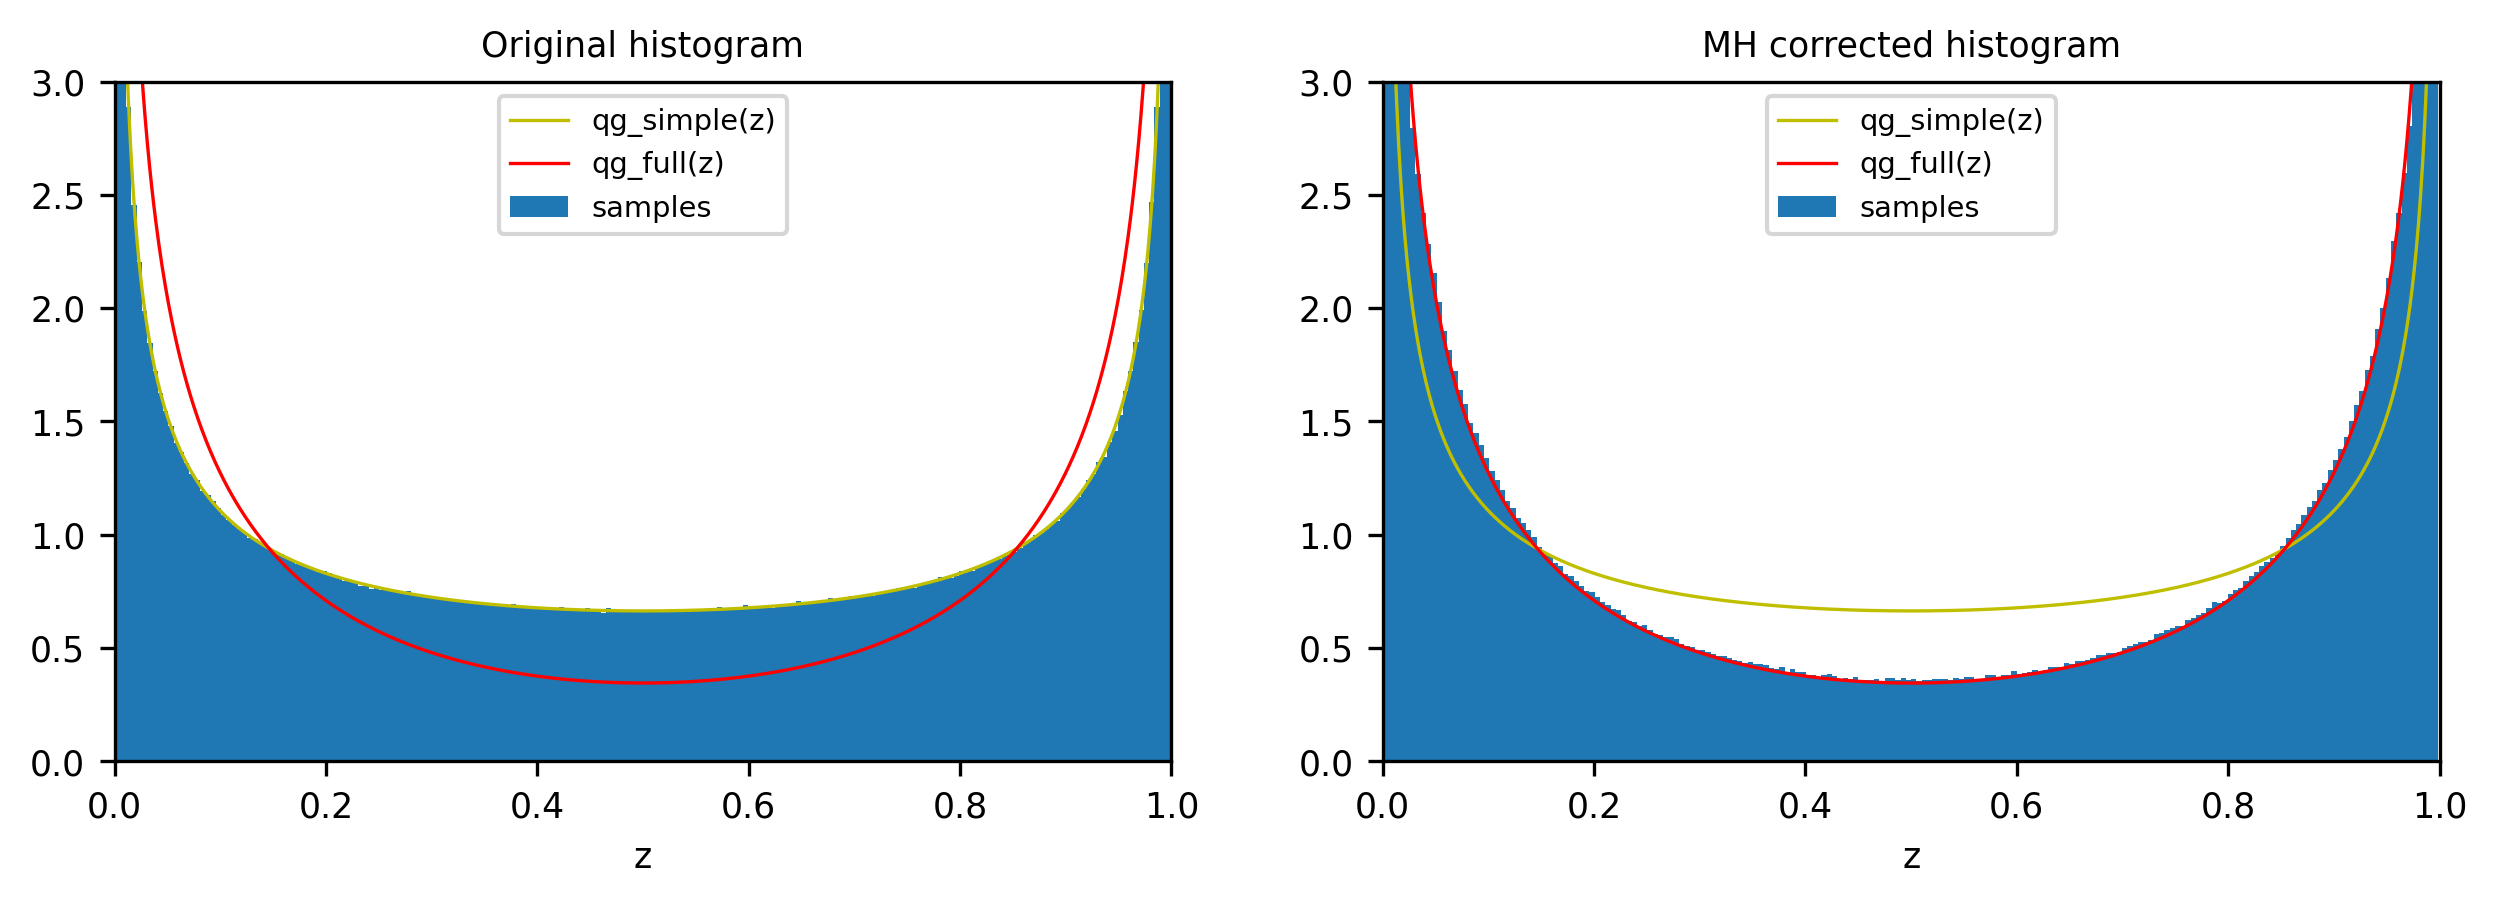
\includegraphics[width=15cm]{pictures/plots/Metropolis-Hastings/MH_medium_qg.png}
    \caption{Probability density of the medium \(\mathcal{K}_{qg}\) splitting function, compared to the histogram of the dummy splitting function, and the Metropolis-Hastings corrected results. Simulated with \(5,000,000\) points, and an acceptance rate of \(0.71\).}
    \label{fig: MH_corrected_k_qg_medium_splitting}
\end{figure}

\subsection*{The \(qq\) vertex}
Finally we have the gq vertex, of \autoref{eqn: medium_full_splittingfunctions_qq}. From this we might try a dummy function such as
\begin{align}
    \mathcal{K}_{qq}^{\text{dummy}}(z) &= \frac{4}{z^{1/2} (1-z)^{3/2}}
\end{align}
whose integral is
\begin{align}
    \int \mathcal{K}_{qq}^{\text{dummy}}(z)\,dz = \int \frac{4}{z^{1/2}(1-z)^{3/2}} \,dz &= \frac{8 \sqrt{z}}{\sqrt{1-z}}.
\end{align}
And we can solve \autoref{eqn: energyfraction_function_R}
\begin{align}
    \mathcal{R}\int_\epsilon^{1-\epsilon} \mathcal{K}_{qq}^{\text{dummy}}(z)\,dz  &= \int_\epsilon^{y} \mathcal{K}_{qq}^{\text{dummy}}(z)\,dz  \nonumber\\
    \mathcal{R}\int_\epsilon^{1-\epsilon} \mathcal{K}_{qq}^{\text{dummy}}(z)\,dz  &= \frac{8\sqrt{y}}{\sqrt{1-y}} - \frac{8\sqrt{\epsilon}}{\sqrt{1-\epsilon}} \nonumber\\
    \frac{\mathcal{R}}{8} \int_\epsilon^{1-\epsilon} \mathcal{K}_{qq}^{\text{dummy}}(z)\,dz + \frac{\sqrt{\epsilon}}{\sqrt{1-\epsilon}} &= \frac{\sqrt{y}}{\sqrt{1-y}}
\end{align}
setting \(a = \frac{\mathcal{R}}{8} \int_\epsilon^{1-\epsilon} \mathcal{K}_{qq}^{\text{dummy}}(z)\,dz + \frac{\sqrt{\epsilon}}{\sqrt{1-\epsilon}}\), we can again solve for \(y\),
\begin{align} \label{eqn: sampling_p_qqg_medium}
    y &= \frac{a^2}{1 + a^2}.
\end{align}
Implementing \autoref{eqn: sampling_p_qqg_medium} into the MH algorithm, we will obtain the distribution given in \autoref{fig: MH_corrected_k_qq_medium_splitting}.
\begin{figure}[hb]
    \centering
    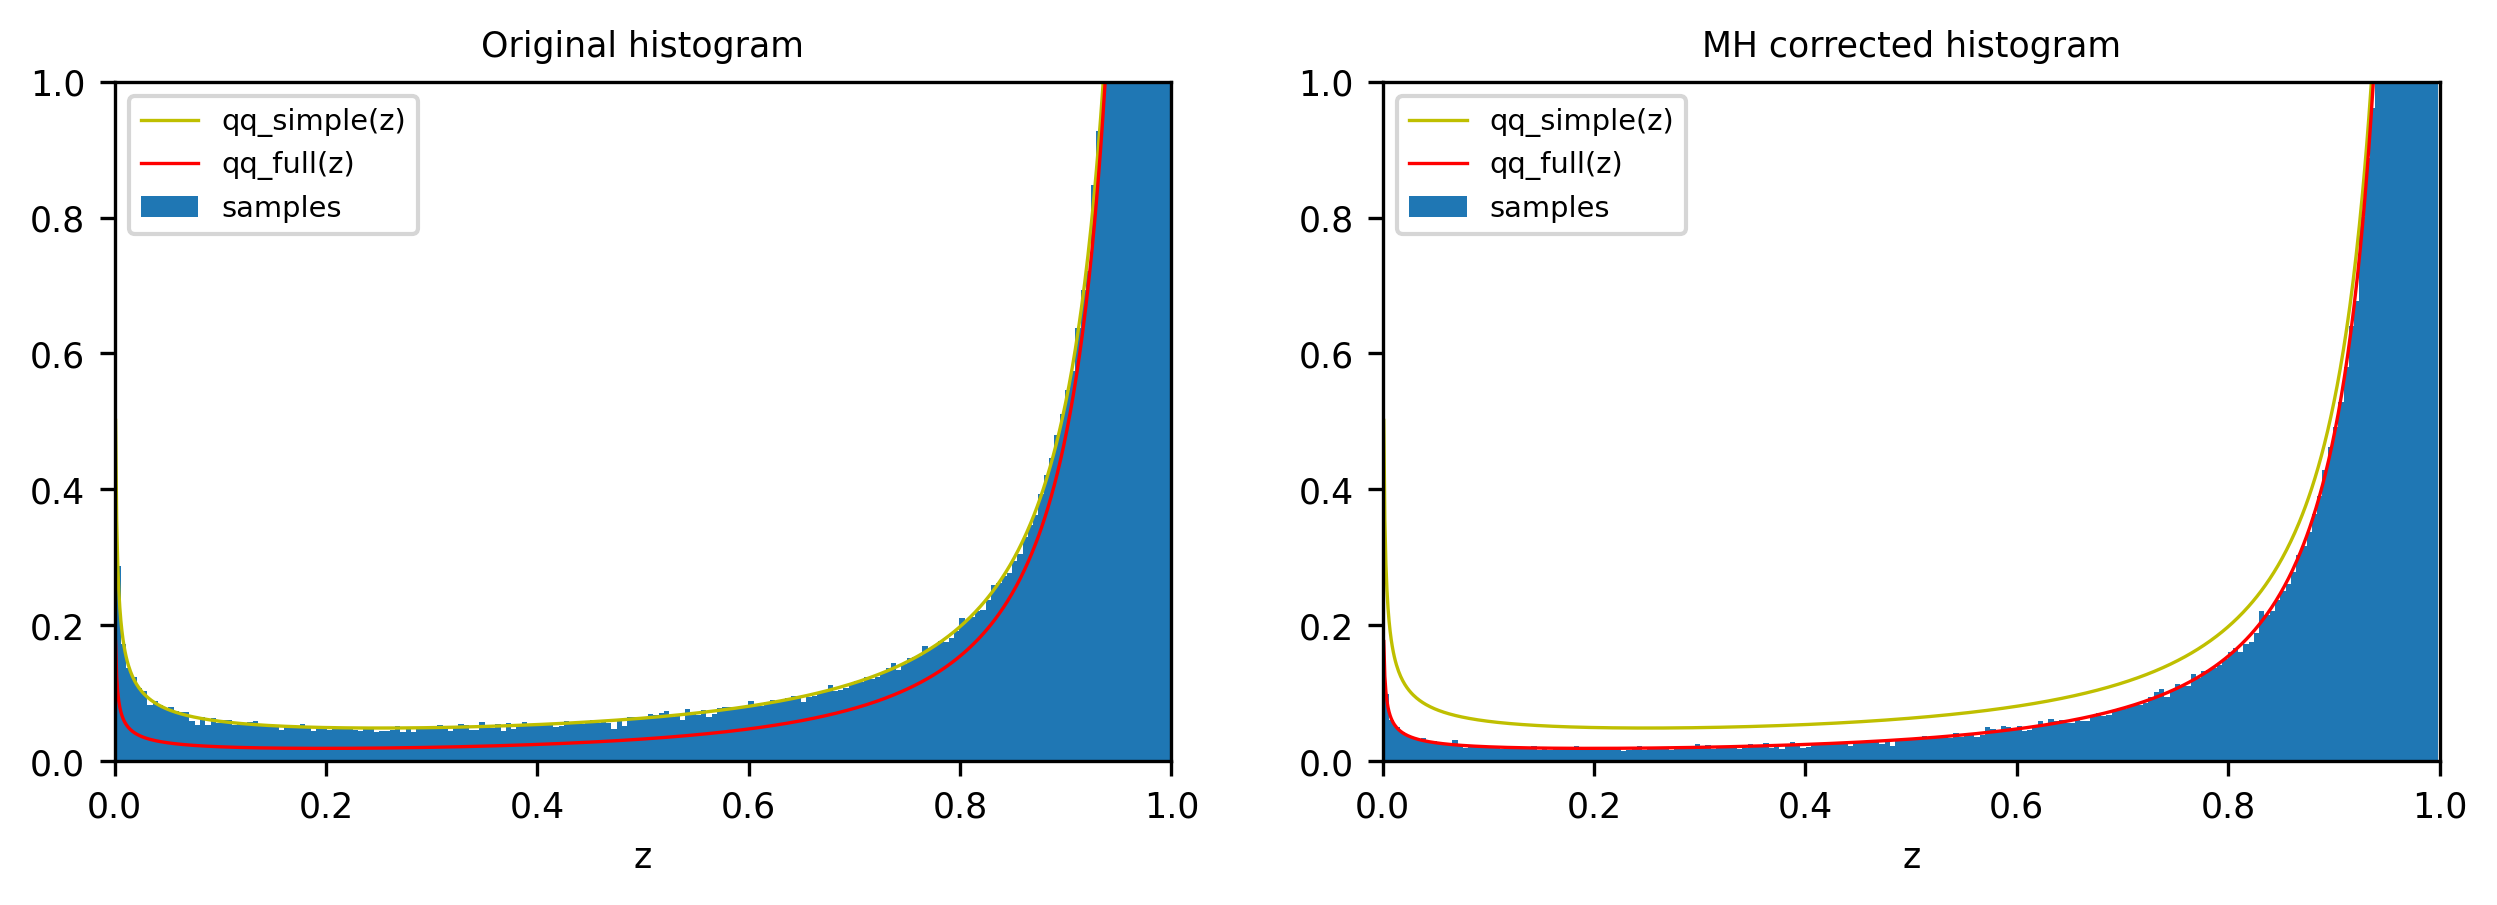
\includegraphics[width=15cm]{pictures/plots/Metropolis-Hastings/MH_medium_qq.png}
    \caption{Probability density of the medium \(\mathcal{K}_{qq}\) splitting function, compared to the histogram of the dummy splitting function, and the Metropolis-Hastings corrected results. Simulated with \(1,000,000\) points, and an acceptance rate of \(0.82\).}
    \label{fig: MH_corrected_k_qq_medium_splitting}
\end{figure}

\end{document}